\documentclass[12pt, a4paper]{report}

% -- Idioma --
\usepackage[spanish]{babel}
% -- Codificación y Fuentes --
\usepackage[utf8]{inputenc}
\usepackage[T1]{fontenc}
\usepackage{titlesec}
\usepackage{url}
\titleformat{\chapter}
  {\normalfont\huge\bfseries}
  {}
  {0pt}
  {}
\titlespacing*{\chapter}{0pt}{20pt}{20pt}
\usepackage{ulem}
\normalem
% --- Interlineado y párrafos ---
\usepackage{parskip}
\setlength{\parindent}{0pt}  
% -- Hipervínculos --
\usepackage[hidelinks]{hyperref}
\usepackage{tocloft}
\renewcommand{\cftchapleader}{\cftdotfill{\cftdotsep}}
% --- Gráficos ---
\usepackage{graphicx}
\graphicspath{{../assets/}}
% -- Márgenes --
\usepackage{geometry}
\geometry{
  top=2.5cm, bottom=2.5cm,
  left=3cm, right=3cm
}
% --- Encabezados y pies de página ---
\usepackage{fancyhdr}
\pagestyle{fancy}
\fancyhf{}
\fancyhead[R]{\footnotesize\textit{Desarrollo de aplicación de equivalencias farmacéuticas internacional - \rightmark}}
\fancyfoot[C]{\thepage}
\renewcommand{\headrulewidth}{0.4pt}
\renewcommand{\sectionmark}[1]{\markright{#1}}
\usepackage{setspace}

% ============================================================
\begin{document}
% ============================================================

% --- Portada ---
\begin{titlepage}
    \centering
    \vspace*{1.5cm}

    {\fontsize{40}{48}\selectfont Universida\textsubscript{de}Vigo}

    \vspace{1cm}
    {\large\textsc{Escola Superior de Enxeñaría Informática}}

    \vspace{3cm}
    Memoria do Traballo de Fin de Grao que presenta

    \vspace{0.5cm}
    {\Large\textbf{D. Marcelo Antonio Veliz Ossandon}}

    \vspace{0.5cm}
    para a obtención do Título de Graduado en Enxeñaría Informática

    \vspace{1.5cm}
    {\large\textbf{Desarrollo de aplicación de equivalencias farmacéuticas internacional}}

    \vfill

    \begin{flushleft}
        Xullo, 2026

        \vspace{0.4cm}
        \textbf{Traballo de Fin de Grao Nº}: 25/26-6 \\
        \textbf{Titor/a:} Eva María Lorenzo Iglesias \\
        \textbf{Área de coñecemento:} Linguaxes e Sistemas Informáticos \\
        \textbf{Departamento:} Informática
    \end{flushleft}
\end{titlepage}

% --- Numeración romana para páginas preliminares ---
\pagenumbering{roman}
\setcounter{page}{1}
\thispagestyle{empty}

% --- Índice de contenidos ---
\selectlanguage{spanish}
\renewcommand{\contentsname}{Índice de Contenidos}
\tableofcontents
\newpage

% --- Índice de ilustraciones ---
\renewcommand{\listfigurename}{Índice de Ilustraciones}
\listoffigures
\newpage

% --- Índice de tablas ---
\renewcommand{\listtablename}{Índice de Tablas}
\listoftables
\newpage

% --- Numeración arábiga para el cuerpo principal ---
\pagenumbering{arabic}
\setcounter{page}{1}

% ==================== Introducción ==========================
\chapter{Introducción}
% TODO: Añadir texto
\newpage
% ============================================================

% ======================= Objetivos ==========================
\chapter{Objetivos}
% TODO: Añadir texto
\newpage
% ============================================================

% ======================== Resumen ===========================
\chapter{Resumen}
% TODO: Añadir texto
\newpage
% ============================================================

% ================ Planificación y Seguimiento ===============
\chapter{Planificación y Seguimiento}
% TODO: Añadir texto
\newpage
% ============================================================

% ======================== Arquitectura ======================
\chapter{Arquitectura}
Para la implementación del sistema, se ha optado por el uso de una \textbf{Arquitectura desacoplada de tres niveles}. Esta se divide en: 
\uline{nivel de presentación} siendo este la interfaz de usuario que estará plasmada en una aplicación Android, \uline{nivel de aplicación} 
con la lógica de negocio para el Backend API, y, \uline{nivel de datos} que contendrá la información de los medicamentos almacenados en una base 
de datos relacional\cite{1}.

El motivo por el cual se está utilizando este tipo de arquitectura es por la flexibilidad que brinda a la hora de separar la lógica del \textit{frontend} 
y \textit{backend} del sistema, permitiendo la implementación de cada una en diferentes lenguajes de programación siendo así más sencillo porque permite 
que el desarrollo de cada nivel sea simultáneo y asegura la escalabilidad de cada uno sin afectar al resto del sistema\cite{1}.

\begin{figure}[h]
    \centering
    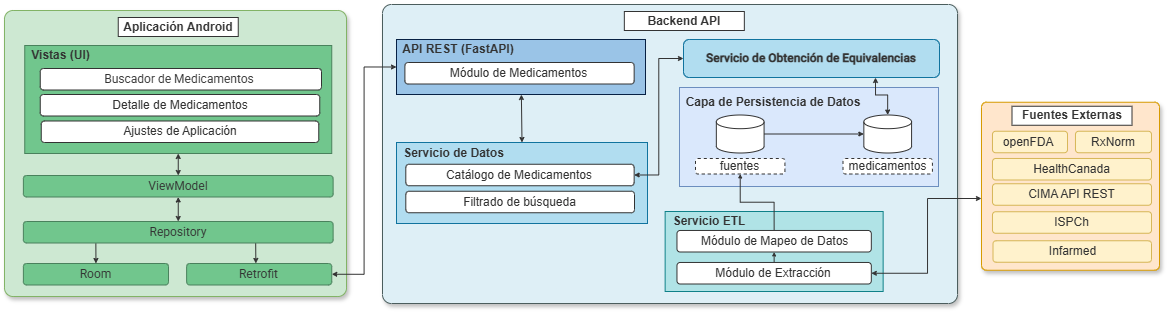
\includegraphics[width=\textwidth]{Diagrama_Arquitectura.png}
    \caption{Arquitectura del Sistema para la Aplicación}
    \label{fig:arquitectura}
\end{figure}

\section{Nivel de Presentación}

Dentro del nivel de presentación, se disponen los elementos necesarios para la interfaz de usuario de la aplicación:

\begin{itemize}
    \item \textbf{Vistas}: Las pantallas que verán los usuarios durante la navegación dentro de la app, donde tendremos elementos como la pantalla principal de la aplicación con el buscador, la información y equivalencias de un medicamento, etc.
    \item \textbf{ViewModel}: Capa intermedia entre interfaz y lógica de app haciendo de intermediario entre su comunicación.
    \item \textbf{Repository}: Actúa como la única fuente de verdad para la obtención de datos en la aplicación. Su objetivo principal es abstraer el origen de los datos a las capas superiores, resolviendo y orquestando las peticiones de red hacia el servidor y abstrayendo la complejidad técnica del consumo de la API o el almacenamiento local.
\end{itemize}

\section{Nivel de Aplicación}

Este nivel alberga la lógica de negocio central de la solución y uno intermediario entre la aplicación móvil y el modelo de datos. Está compuesto por el Backend API, el cual expone y procesa las funcionalidades del sistema mediante los siguientes componentes:

\begin{itemize}
    \item \textbf{API REST}: Funciona como el punto de entrada de todas las comunicaciones externas. Expone diversos \textit{endpoints} HTTP que permiten al nivel de presentación enviar peticiones (como por ejemplo, búsquedas por principio activo o peticiones de equivalencias) y recibir una respuesta estructurada en formato JSON.

    \item \textbf{Servicios de Datos}: Capa intermediaria dentro del Backend que asume la responsabilidad de procesar y aplicar las reglas de negocio. Estos servicios interpretan lo que llega desde la API REST, interactúan con la capa de persistencia para extraer la información y preparan/formatean los registros en objetos de respuesta de forma limpia y manejable para el cliente.

    \item \textbf{Servicio ETL (Extract, Transform, Load)}: Módulo integral encargado de la ingesta de información. Su cometido es extraer los datos en crudo de los distintos países, aplicar transformaciones complejas tales como la limpieza de cadenas, recolección de códigos ATC, formas farmacéuticas, etc. y cargar finalmente la información unificada y estandarizada en el esquema de la base de datos de producción.

    \item \textbf{Servicio de Obtención de Equivalencias}: Es el módulo algorítmico responsable de cruzar los medicamentos de un país de origen con los equivalentes de un país destino. Lleva a cabo el emparejamiento basándose primordialmente en una coincidencia exacta de los códigos ATC, y alternativamente como medida de respaldo, buscando coincidencias en los principios activos del propio fármaco.
\end{itemize}

\section{Nivel de Datos}

El nivel de datos se encarga de todo lo relativo al almacenamiento robusto e íntegro de la información, permitiendo la persistencia a largo plazo y la recopilación de registros:

\begin{itemize}
    \item \textbf{Capa de Persistencia}: Almacena la información relevante en relación a los datos del sistema, materializada en un Sistema de Gestión de Bases de Datos Relacional. Esta base de datos dispone de dos esquemas principales:
    \begin{itemize}
        \item \textit{Fuentes}: Almacena los datos crudos de los medicamentos provenientes de las fuentes externas.
        \item \textit{Medicamentos}: Almacena los datos normalizados de los medicamentos del sistema una vez procesado el servicio ETL.
    \end{itemize}

    \item \textbf{Fuentes Externas}: Conforman los registros de medicamentos en crudo y repositorios ajenos al sistema de los cuales se parte para poblar la capa de persistencia mediante el servicio ETL: \textbf{\textit{AEMPS}} proporciona los datos de España mediante la API oficial de CIMA. \textbf{\textit{ISPCh}} contiene una base de datos pública para Chile y de igual manera \textbf{\textit{INFARMED}} proporciona las suya para los de Portugal\cite{2}\cite{3}\cite{4}\cite{5}.

    \textbf{\textit{Health Canada}} al igual que España tiene su propia API con la base de datos de medicamentos para Canadá. En Estados Unidos se utilizan dos fuentes: \textbf{\textit{OpenFDA}} con los datos comerciales de los medicamentos y \textbf{\textit{RxNorm}} con la información técnica como los códigos ATC o Principios Activos\cite{6}\cite{7}\cite{8}.
\end{itemize}

\newpage
% ============================================================

% ==== Tecnologías e integración de productos de terceros ====
\chapter{Tecnologías Utilizadas}
% TODO: Añadir texto
\newpage
% ============================================================

% ========== Especificación y Análisis de Requisitos =========
\chapter{Especificación}
A continuación, se definen las historias de usuario para las funcionalidades clave de la aplicación cuyos requisitos deben cumplirse obligatoriamente:

\section{Historias de Usuario}
\noindent\textbf{Identificador:} HU-01 \\
\textbf{Título:} Búsqueda de Medicamentos \\
\textbf{Prioridad:} Alta \\
\textbf{Descripción:}
\begin{itemize}
    \item Como Usuario, quiero tener disponible un buscador en la pantalla principal de la aplicación para poder realizar las búsquedas de los distintos medicamentos que estén almacenados en la aplicación.
\end{itemize}
\textbf{Criterios de aceptación:}
\begin{itemize}
    \item Como mínimo, la información de dicho medicamento tiene que existir dentro de la base de datos de la aplicación.
    \item El buscador debe permitir buscar tanto por nombre comercial (ej. ``Gelocatil''), por principio activo (ej. ``Paracetamol'') o por código ATC (ej. ``N02BE01'').
    \item Si no hay resultados, se debe mostrar un mensaje claro indicando que ``No se han encontrado medicamentos''.
\end{itemize}

\vspace{0.5cm}
\noindent\textbf{Identificador:} HU-02 \\
\textbf{Título:} Filtrado avanzado de Búsquedas \\
\textbf{Prioridad:} Media \\
\textbf{Descripción:}
\begin{itemize}
    \item Como Usuario, a la hora de realizar búsquedas quiero poder hacer filtrado de la información de un medicamento acotado por características como laboratorio de fabricación, dosaje, vía de administración, etc. para poder facilitar la búsqueda de un medicamento en concreto.
\end{itemize}
\textbf{Criterios de aceptación:}
\begin{itemize}
    \item El usuario debe poder aplicar múltiples filtros simultáneamente (ej. Vía de administración + Forma farmacéutica).
    \item Los selectores de filtros solo deben mostrar opciones asociadas a los atributos que posee el medicamento en la base de datos.
    \item Si la combinación de filtros no arroja ningún resultado, se debe mostrar un mensaje al usuario indicando ``No se han encontrado coincidencias''.
    \item Debe haber un botón en la aplicación para limpiar los filtros.
\end{itemize}

\vspace{0.5cm}
\noindent\textbf{Identificador:} HU-03 \\
\textbf{Título:} Visualización detallada de un Medicamento \\
\textbf{Prioridad:} Media \\
\textbf{Descripción:}
\begin{itemize}
    \item Como Usuario, quiero poder observar los detalles técnicos de un medicamento para conocer información del mismo ya sea el número identificativo local de este (ej. el DIN en Canadá), laboratorio fabricante, dosaje de medicamento, código ATC, principio activo, etc.
\end{itemize}
\textbf{Criterios de aceptación:}
\begin{itemize}
    \item Entre los detalles, los atributos imprescindibles son: Nombre Comercial, Principio Activo, Código ATC (en caso de tener), País de Origen y Laboratorio.
    \item Si algún dato no está disponible en la base de datos (ej. En el caso de Chile que no tiene datos específicos de Dosaje por ejemplo), la interfaz mostrará un texto en dicho campo como ``No Disponible''.
\end{itemize}

\vspace{0.5cm}
\noindent\textbf{Identificador:} HU-04 \\
\textbf{Título:} Comparación de Medicamentos Internacionales \\
\textbf{Prioridad:} Alta \\
\textbf{Descripción:}
\begin{itemize}
    \item Como Usuario, además de poder ver la información detallada de un medicamento necesito poder ver la equivalencia entre un medicamento de cierto país de origen con el medicamento de otro país, con la finalidad de conocer alternativas al medicamento del país de origen dentro del país buscado.
\end{itemize}
\textbf{Criterios de aceptación:}
\begin{itemize}
    \item Al seleccionar un medicamento de origen, el sistema debe ser capaz de listar sus equivalencias en el país destino basándose en una coincidencia exacta del código ATC.
    \item En caso de que un medicamento carezca de código ATC en la base de datos, el sistema debe realizar el cruce internacional utilizando la coincidencia del Principio Activo.
    \item La interfaz debe indicar el grado de similitud, indicar si poseen mismo código ATC o si la equivalencia se basa únicamente en el principio activo.
\end{itemize}

\vspace{0.5cm}
\noindent\textbf{Identificador:} HU-05 \\
\textbf{Título:} Selector de Idiomas \\
\textbf{Prioridad:} Media \\
\textbf{Descripción:}
\begin{itemize}
    \item Como Usuario, necesito tener la opción de poder cambiar el idioma de la aplicación para poder realizar un mejor uso de la misma obteniendo las interfaces en mi idioma preferido.
\end{itemize}
\textbf{Criterios de aceptación:}
\begin{itemize}
    \item El sistema debe soportar, como mínimo, los idiomas Español e Inglés.
    \item El cambio de idioma debe aplicarse instantáneamente en la interfaz sin necesidad de reiniciar la aplicación.
\end{itemize}

\vspace{0.5cm}
\noindent\textbf{Identificador:} HU-06 \\
\textbf{Título:} Cambiar Aspecto \\
\textbf{Prioridad:} Media \\
\textbf{Descripción:}
\begin{itemize}
    \item Como Usuario, quiero que la interfaz de la aplicación se adapte al aspecto que tenga mi dispositivo, ya sea modo claro o modo oscuro, por lo que debo tener una opción para poder cambiarlo.
\end{itemize}
\textbf{Criterios de aceptación:}
\begin{itemize}
    \item La aplicación debe detectar automáticamente si el dispositivo usado está en modo claro u oscuro y aplicar el tema correspondiente.
    \item Los temas que se vayan emplear, tanto para modo claro como modo oscuro, deben permitir la clara visualización de la información de los medicamentos.
\end{itemize}

\section{Casos de Uso}

\begin{figure}[h]
    \centering
    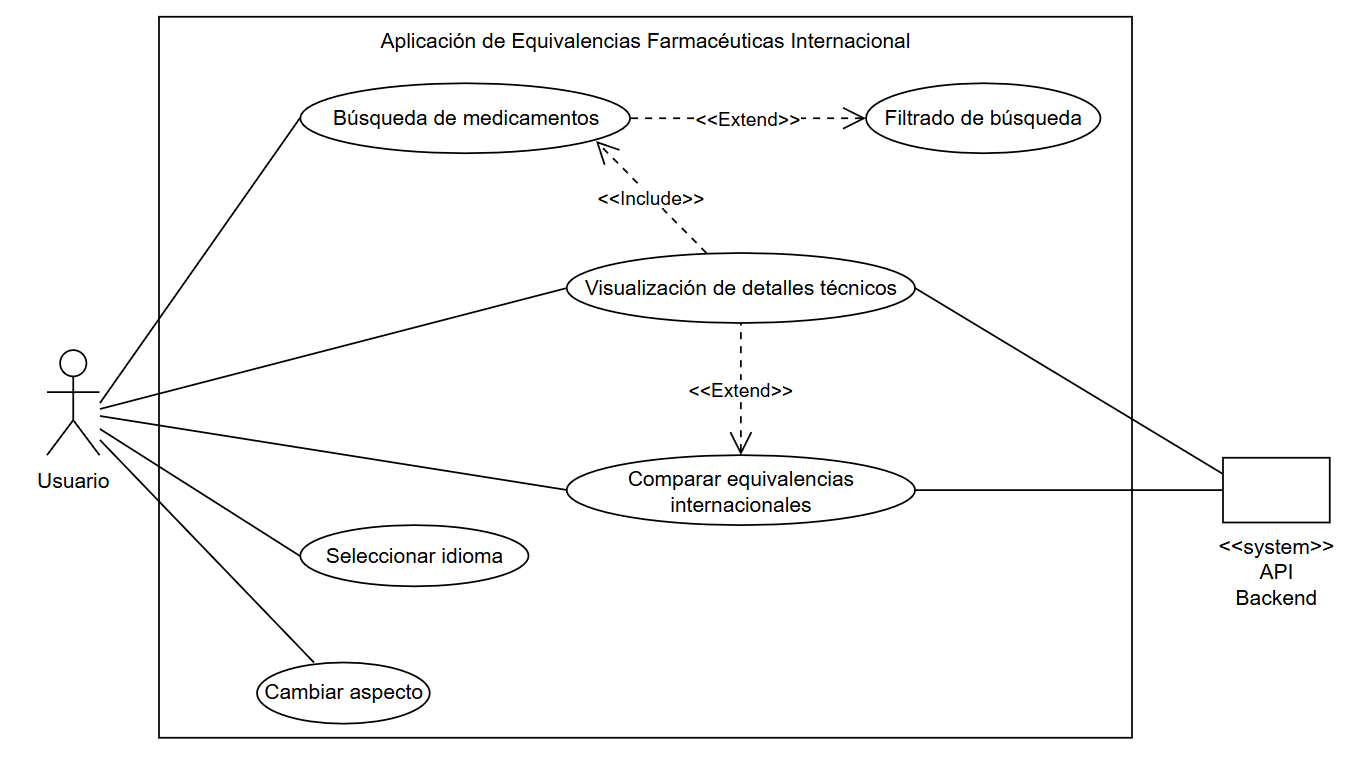
\includegraphics[width=0.85\textwidth]{Diagrama_Casos_de_Uso.png}
    \caption{Diagrama de casos de uso de la Aplicación}
    \label{fig:casos_uso}
\end{figure}

\newpage
% ============================================================

% =================== Diseño de Software =====================
\chapter{Diseño de Software}
A continuación se detalla el diseño de las diferentes piezas de software que componen la solución. Debido a la naturaleza modular de esta aplicación, 
este diseño se ha dividido en distintos bloques lógicos que abarcan la ingesta de información, la gestión de persistencia y las funcionalidades expuestas 
hacia la capa de presentación.

\section{Base de Datos}
El diseño de la base de datos es fundamental para garantizar la integridad, estructuración y el acceso eficiente a la información médica internacional de 
los medicamentos.

La estructura del esquema de persistencia está definido por los scripts SQL dentro del directorio \textit{\path{modulo_datos/database/}} que se divide 
lógicamente en dos esquemas principales:

\begin{itemize}
    \item \textbf{Esquema de \textit{fuentes}}: Actúa como área de \textit{staging} o zona de aterrizaje transitoria para los datos crudos extraídos directamente de las agencias gubernamentales. Alberga tablas independientes sin relaciones de integridad entre sí para cada país (\texttt{spain\_med}, \texttt{chile\_med}, \texttt{canada\_med}, \texttt{usa\_med} y \texttt{portugal\_med}).

    \item \textbf{Esquema de \textit{medicamentos}}: Representa el núcleo del modelo relacional normalizado. Aquí es donde convergen de forma estandarizada todos los datos ya limpios y listos para ser consumidos.
\end{itemize}

\begin{figure}[h]
    \centering
    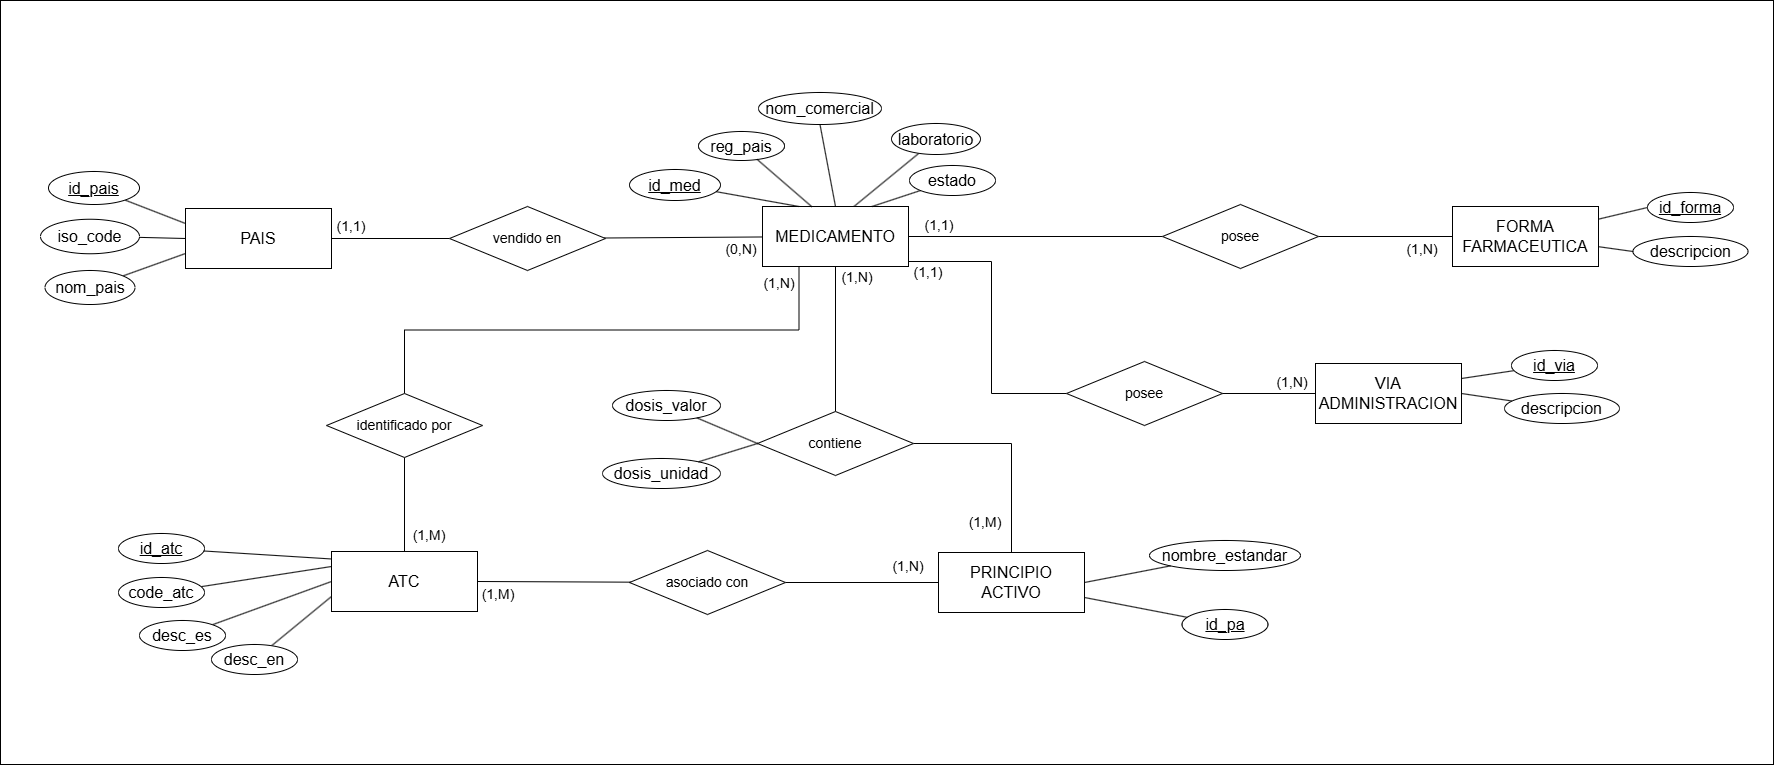
\includegraphics[width=\textwidth]{Diagrama_MER.png}
    \caption{Diagrama Entidad-Relación (MER) del esquema de Medicamentos}
    \label{fig:diagrama_mer}
\end{figure}

El modelo relacional de los medicamentos está conformado por \textbf{\uline{tres elementos clave}}:

\begin{itemize}
    \item \textbf{Tablas Maestras}: Entidades fuertes y descriptivas que albergan valores estandarizados: \texttt{pais}, \texttt{atc}, \texttt{principio\_activo}, \texttt{forma\_farmaceutica} y \texttt{via\_administracion}.

    \item \textbf{Entidad Principal (\texttt{medicamento})}: Almacena los atributos fundamentales e identificativos inherentes a cada fármaco (\textbf{nombre comercial}, \textbf{laboratorio} fabricante y \textbf{número de registro}) y se nutre mediante claves foráneas de origen, forma y vía correspondiente.

    \item \textbf{Tablas Intermedias de Relación (N:M)}: Estructuras relacionales vitales para soportar la multiplicidad del dominio médico. Destacan la tabla \textbf{contiene}, que vincula con uno o varios de sus principios activos, \textbf{identificado\_por}, esta asocia un medicamento con sus códigos ATC, y por último, \textbf{asociado\_con} que enlaza los principios activos genéricos con el estándar resolutivo ATC.
\end{itemize}

\section{Módulo de ETL}
El módulo de ETL (Extracción, Transformación y Carga) es el componente responsable de centralizar, estandarizar y poblar la base de datos de producción con el catálogo internacional de medicamentos.

\begin{figure}[h]
    \centering
    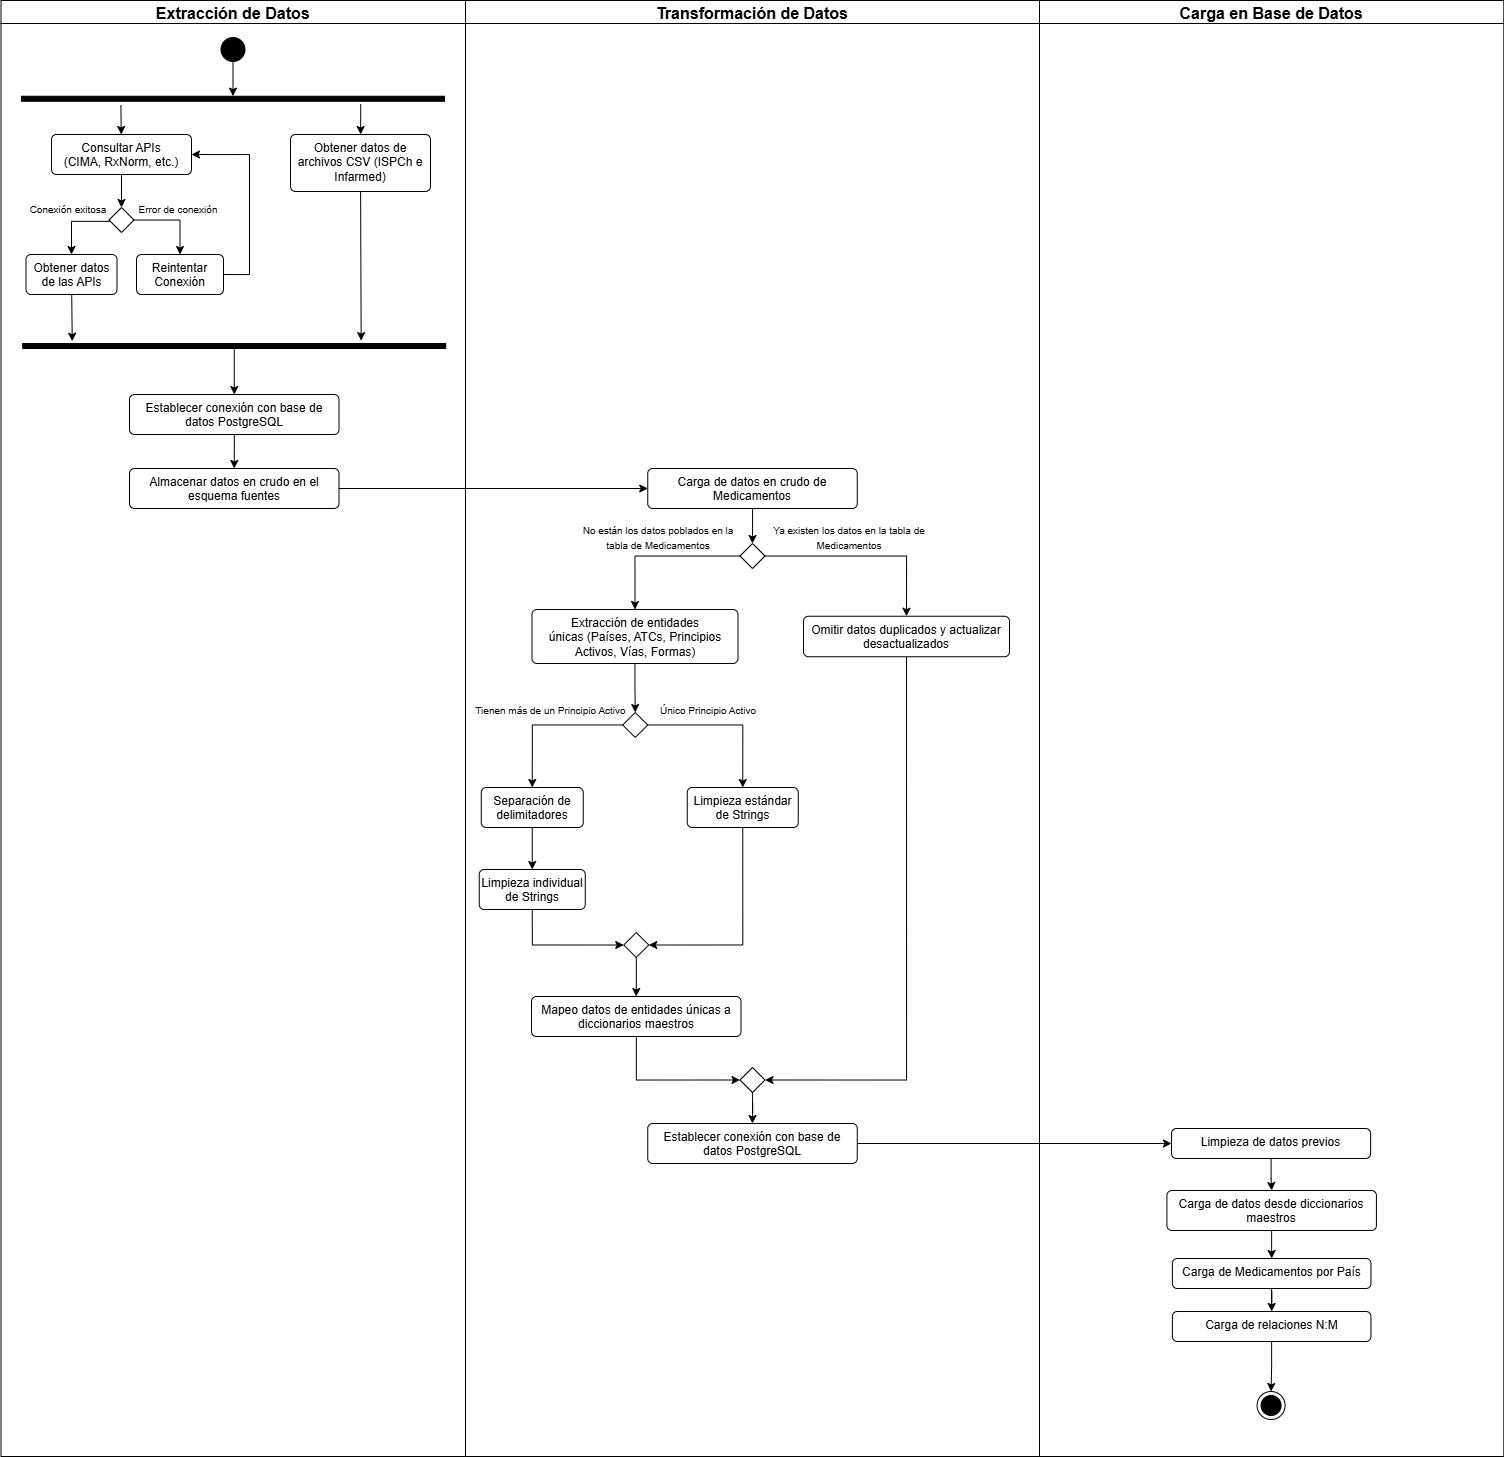
\includegraphics[width=\textwidth]{Diagrama_Actividad_ETL.png}
    \caption{Diagrama de Actividad sobre proceso ETL}
    \label{fig:diagrama_etl}
\end{figure}

\subsection{Extracción de Datos}
Consiste en la obtención inicial de los datos a través de las diversas fuentes externas. Por un lado, se consultan de manera automatizada las \textbf{APIs oficiales}, por ejemplo CIMA o RxNorm, manejando posibles errores de conexión y reintentos de consulta. Para las fuentes que no disponen de este servicio (Chile y Portugal), se obtienen los datos procedentes de \textbf{archivos CSV}. Toda información recién adquirida se extrae y se almacena en un esquema propio de \textit{fuentes} en la base de datos.

Para la extracción de datos se implementaron los scripts en Python dentro del directorio \textit{\path{modulo_datos/scripts/fuentes_externas}}:

\begin{itemize}
    \item \textit{\texttt{spain\_med.py}}: Extrae los medicamentos de \textbf{España} desde la API de CIMA.
    \item \textit{\texttt{chile\_med.py}}: Extrae los medicamentos de \textbf{Chile} desde el CSV con los datos proporcionados por el ISPCh.
    \item \textit{\texttt{portugal\_med.py}}: Extrae los medicamentos de \textbf{Portugal} desde el CSV con los datos proporcionados por INFARMED.
    \item \textit{\texttt{canada\_med.py}}: Extrae los medicamentos de \textbf{Canadá} desde la API oficial con los datos del Drug Product Database de Health Canada.
    \item \textit{\texttt{usa\_fda.py}}: Extrae los \uline{datos comerciales} de los medicamentos de \textbf{Estados Unidos} desde la API de Drugs@FDA proporcionado por openFDA.
    \item \textit{\texttt{usa\_rxnorm.py}}: Extrae los \uline{datos técnicos} que contienen los \textbf{códigos ATC y principios activos de los medicamentos estadounidenses} desde la API de RxNorm.
\end{itemize}

\subsection{Transformación de Datos}
En este paso se toma la carga de datos en crudo y se evalúa si dichos datos ya se encuentran en el sistema. En caso afirmativo, se omiten duplicados y se actualizan los desfasados. De tratarse de un registro nuevo, se procede a extraer sus entidades únicas: \textit{Países}, \textit{códigos ATC}, \textit{Principios Activos}, \textit{Vías de Administración} y \textit{Formas Farmacéuticas}.

Además, si se determina que conforma más de un principio activo se somete a una limpieza y estandarización más básica. Como cierre, todos estos elementos transformados se mapean estructurando diccionarios maestros en memoria.

Todo este proceso se implementó en el script Python \textbf{\texttt{01\_load\_diccionarios.py}} ubicado en el directorio \textit{\path{modulo_datos/scripts/etl}}.

\subsection{Carga en Base de Datos}
Representa la última etapa de consolidación hacia las tablas relacionales finales. Este proceso de carga está implementado en dos scripts en Python que se ejecutan secuencialmente posterior al de transformación de datos dentro del directorio \textit{\path{modulo_datos/scripts/etl}}:

\begin{itemize}
    \item \textbf{\texttt{02\_load\_medicamentos.py}}: Se encarga de volcar el volumen más pesado, realizando la carga e inserción completa de la información básica y principal del propio medicamento desglosado por país.

    \item \textbf{\texttt{03\_load\_relaciones.py}}: Por último, se enlazan las partes consolidando las relaciones de tipo N:M en la base de datos. De esta manera le permite al sistema cruzar qué medicamentos contienen qué principios activos en determinadas cantidades, posibilitando a su vez, la obtención de equivalencias internacionales.
\end{itemize}

\section{Backend API}
% TODO: Añadir texto
\section{Aplicación Android}
% TODO: Añadir texto

\newpage
% ============================================================

% ============= Gestión de Datos e Información ===============
\chapter{Gestión de Datos e Información}
% TODO: Añadir texto
\newpage
% ============================================================

% =================== Pruebas ================================
\chapter{Pruebas}
% TODO: Añadir texto
\newpage
% ============================================================

% ================ Manual de Usuario =========================
\chapter{Manual de Usuario}
% TODO: Añadir texto
\newpage
% ============================================================

% ============== Principales Aportaciones ====================
\chapter{Principales Aportaciones}
% TODO: Añadir texto
\newpage
% ============================================================

% =================== Conclusiones ===========================
\chapter{Conclusiones}
% TODO: Añadir texto
\newpage
% ============================================================

% ==================== Referencias ===========================
\begin{thebibliography}{8}

\bibitem{1}
IBM, ``¿Qué es la arquitectura de tres niveles?'', \textit{IBM Think}. [En línea]. Disponible en: \url{https://www.ibm.com/es-es/think/topics/three-tier-architecture}. [Accedido: 21-mar-2026].

\bibitem{2}
Agencia Española de Medicamentos y Productos Sanitarios (AEMPS), ``\textit{CIMA REST API}'', AEMPS. [En línea]. Disponible en: \url{https://www.aemps.gob.es/apps/cima/docs/CIMA_REST_API.pdf}. [Accedido: 27-ene-2026].

\bibitem{3}
Agencia Española de Medicamentos y Productos Sanitarios (AEMPS), ``\textit{Centro de Información online de Medicamentos de la AEMPS (CIMA)}'', AEMPS. [En línea]. Disponible en: \url{https://cima.aemps.es/cima/publico/home.html}. [Accedido: 28-ene-2026].

\bibitem{4}
Instituto de Salud Pública de Chile (ISP), ``\textit{Instituto de Salud Pública de Chile}'', ISP. [En línea]. Disponible en: \url{https://www.ispch.gob.cl/}. [Accedido: 31-ene-2026].

\bibitem{5}
Autoridade Nacional do Medicamento e Produtos de Saúde (INFARMED), ``\textit{Infarmed -- National Authority of Medicines and Health Products}'', INFARMED. [En línea]. Disponible en: \url{https://www.infarmed.pt/web/infarmed-en}. [Accedido: 02-feb-2026].

\bibitem{6}
Health Canada, ``\textit{Drug Product Database}'', Government of Canada. [En línea]. Disponible en: \url{https://www.canada.ca/en/health-canada/services/drugs-health-products/drug-products/drug-product-database.html}. [Accedido: 05-feb-2026].

\bibitem{7}
U.S. Food and Drug Administration (FDA), ``\textit{Drugs@FDA: FDA-Approved Drugs}'', openFDA. [En línea]. Disponible en: \url{https://open.fda.gov/apis/drug/drugsfda/}. [Accedido: 08-feb-2026].

\bibitem{8}
National Library of Medicine (NLM), ``\textit{RxNorm}'', National Institutes of Health (NIH). [En línea]. Disponible en: \url{https://www.nlm.nih.gov/research/umls/rxnorm/index.html}. [Accedido: 10-feb-2026].

\end{thebibliography}
% ============================================================

% ============================================================
\end{document}
% ============================================================